\documentclass[french]{beamer}

\usepackage[frenchb]{babel}
\usepackage[T1]{fontenc}
\usepackage[utf8]{inputenc}
\usepackage{amsmath}

\usetheme{Hannover}

\title{Reconstitution 3D à partir de photographies : Détection de contour}
\author{}
\date{}

\begin{document}
\setbeamertemplate{caption}{\raggedright\insertcaption\par}

\begin{frame}
	\maketitle
	\vspace{-3cm}
	Extraction de la silhouette\\
	\medskip
	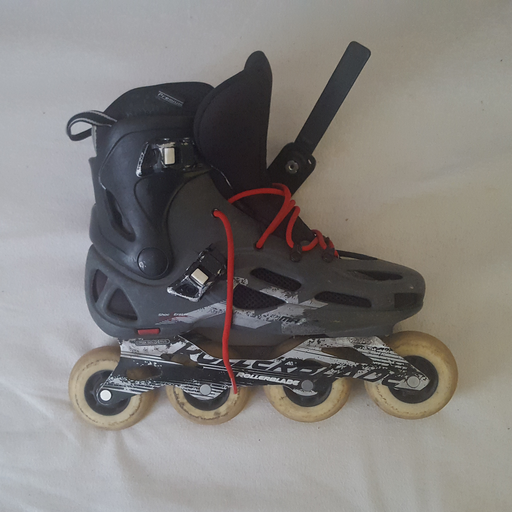
\includegraphics[width=2cm]{images/roller.png} \; 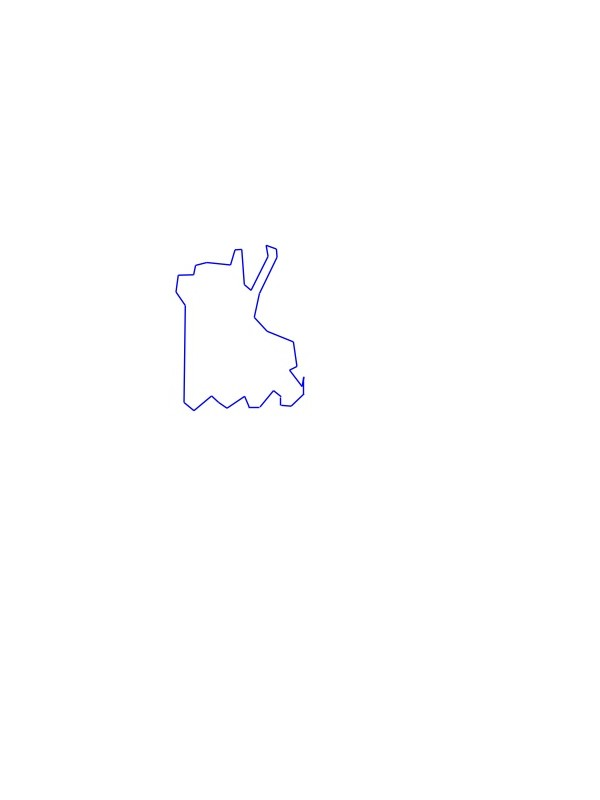
\includegraphics[width=2cm]{images/roller_poly.jpg}\\
	Intersection des silhouettes\\
	\medskip
	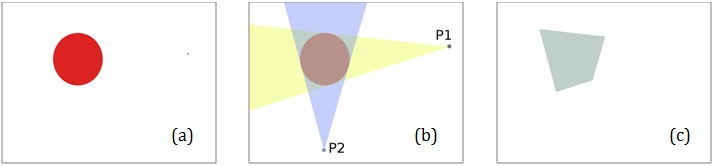
\includegraphics[height=2cm]{images/silhouettes.jpg}
\end{frame}

\begin{frame}
	\frametitle{Choix des Types}
	\textbf{Type} : Flottant-4octet, Complex-8octet
	\smallskip
	\begin{itemize}
		\item Plus rapide : processeur à opérations flottantes
		\item Pas de dépassement : exposant sur 8-bits $\longrightarrow \text{max} =  10^{256}$
	\end{itemize}
	\bigskip
	\textbf{Structure} : \\
	\smallskip
	Tableaux numpy à 5 dimensions : \\
	\begin{tabular}{|c|c|c|c|l|}
		\hline
		1 & 2 & 3 & 4 & 5 \\ \hline
		$dx$ & $dy$ & $x$ & $y$ & $i$ \\ \hline
		\multicolumn{2}{|l|}{index voisinage} & \multicolumn{2}{|l|}{index image} & composantes \\
		\hline
	\end{tabular}
\end{frame}

\begin{frame}
	\frametitle{Complexité}
	\textbf{Temporelle} \\
	\smallskip
	En théorie :
	\begin{itemize}
		\item Opérations vectorielles : GPU. \;\;\; $\longrightarrow$ noté $\nu(n)$
		\item Autres : CPU.
	\end{itemize}
	En pratique :
	\begin{itemize}
		\item Opérations vectorielles : numpy, boucles en C.
		\item Autres : python
	\end{itemize}
	Objectif : Vectoriser au maximum les opérations. \\
	\bigskip
	\textbf{Spatiale} \\
	\smallskip
	Vectorisation $\longrightarrow$ Complexité spatiale très grande :\\
	$\theta(t^2 \cdot n^2) \approx (8\text{octet} \cdot 1000 \cdot 1\text{Mpix} = 8 \text{Gib})$ \\
	\smallskip
	Coût de copie : Relativement élevé $\approx \nu(n^2)$\\
	Manipulation bas niveau du hardware (registres vectorielle du GPU) $\longrightarrow$ rapide
\end{frame}

\begin{frame}
	\frametitle{Procédé Général}
	\tableofcontents
\end{frame}

\section{Espace LAB}

\begin{frame}
	\frametitle{Espace LAB}
	\begin{columns}
		\begin{column}{5cm}
			$$L = \frac{R + G + B}{3}$$
			$$A = \frac{G - R + 255}{2}$$
			$$B = \frac{G - B + 255}{2}$$
		\end{column}
		\begin{column}{5cm}
			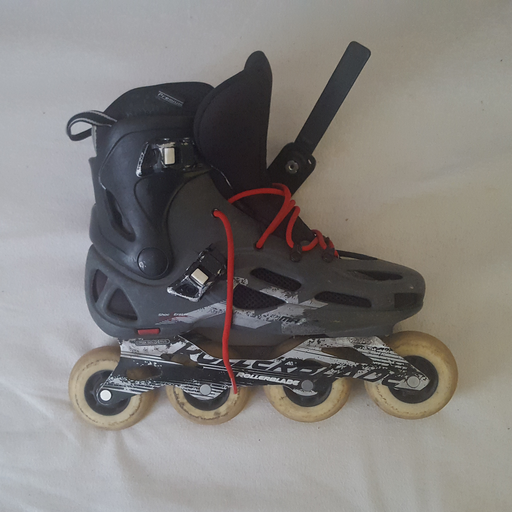
\includegraphics[width=3cm]{images/roller.png}\\
			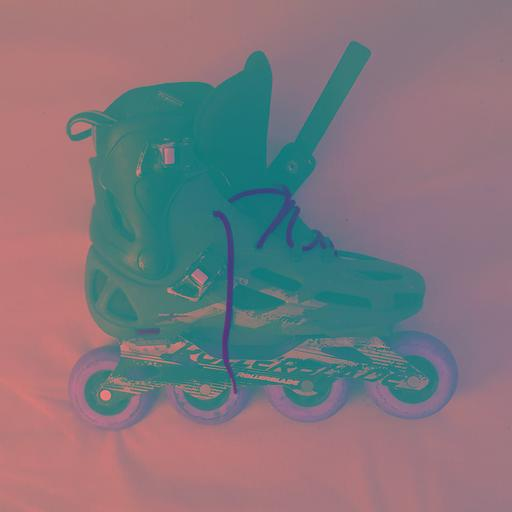
\includegraphics[width=3cm]{images/roller_lab.jpg}
		\end{column}
	\end{columns}
	Complexité : $\theta(\nu(n^2))$
\end{frame}

\section{Filtrage fréquentiel : Texture}

\begin{frame}
	\frametitle{\mbox{1\up{er} Filtrage - Domaine fréquentiel - Texture}}
	\framesubtitle{Procédé}
	\underline{Convolution} par un \textbf{filtre gaussien} $\longleftrightarrow$ \underline{Multiplication} dans le domaine fréquentielle.
	\begin{figure}
		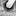
\includegraphics[width=2cm]{images/roller_subim.jpg} \; 
\includegraphics[width=2cm]{images/roller_subimfft.jpg} \;
		
\includegraphics[width=2cm]{images/roller_subimf.jpg} \; 
\includegraphics[width=2cm]{images/roller_subimresp.jpg}\\
		\caption{Sous-image \; - \; Transformée \; - \; Filtre \; - \; Réponse}
	\end{figure}
	\bigskip
	Sommation de tous les pixels $\longrightarrow$ valeur de texture.\\
	\medskip
	Complexité spatiale : $\theta(t^2 \cdot n^2)$
\end{frame}

\begin{frame}
	\frametitle{\mbox{1\up{er} Filtrage - Domaine fréquentiel - Texture}}
	\framesubtitle{Transformée de Fourier}
	Définition :
	\begin{itemize}
		\item Continue :\; $F(f)(s) = \frac{1}{\sqrt{2\pi}} \int_a^b e^{- 2i\pi sx} \cdot f(x) \, \mathrm dx$ \\
		\item Discrete :\; $FD(u)(k) = \frac{1}{\sqrt{N}} \sum\limits_{n = 0}^{n = N - 1} e^{-2i\pi \frac{kn}{N}} \cdot u{n}$
	\end{itemize}
	\medskip
	Propriété de convolution : $u \star v = DF^{-1}(DF(u) \cdot DF(v))$ (Au facteur près)\\
	\medskip
	Complexité temporelle
	\begin{itemize}
		\item Sur un vecteur : $\theta(n \cdot \nu(n))$
		\item Sur une image : $\theta(n \nu(n^2))$
	\end{itemize}
	\medskip
	Complexité spatiale : En place \\
	\medskip
	\textbf{Transformée de Fourier rapide} : Diviser pour régner
	\begin{itemize}
		\item Sur un vecteur : $\theta(\log_2(n)\nu(n))$
		\item Sur une image : $\theta(\log_2(n)\nu(n^2))$
	\end{itemize}
\end{frame}

\begin{frame}
	\frametitle{\mbox{1\up{er} Filtrage - Domaine fréquentiel - Texture}}
	\framesubtitle{Exemples}
	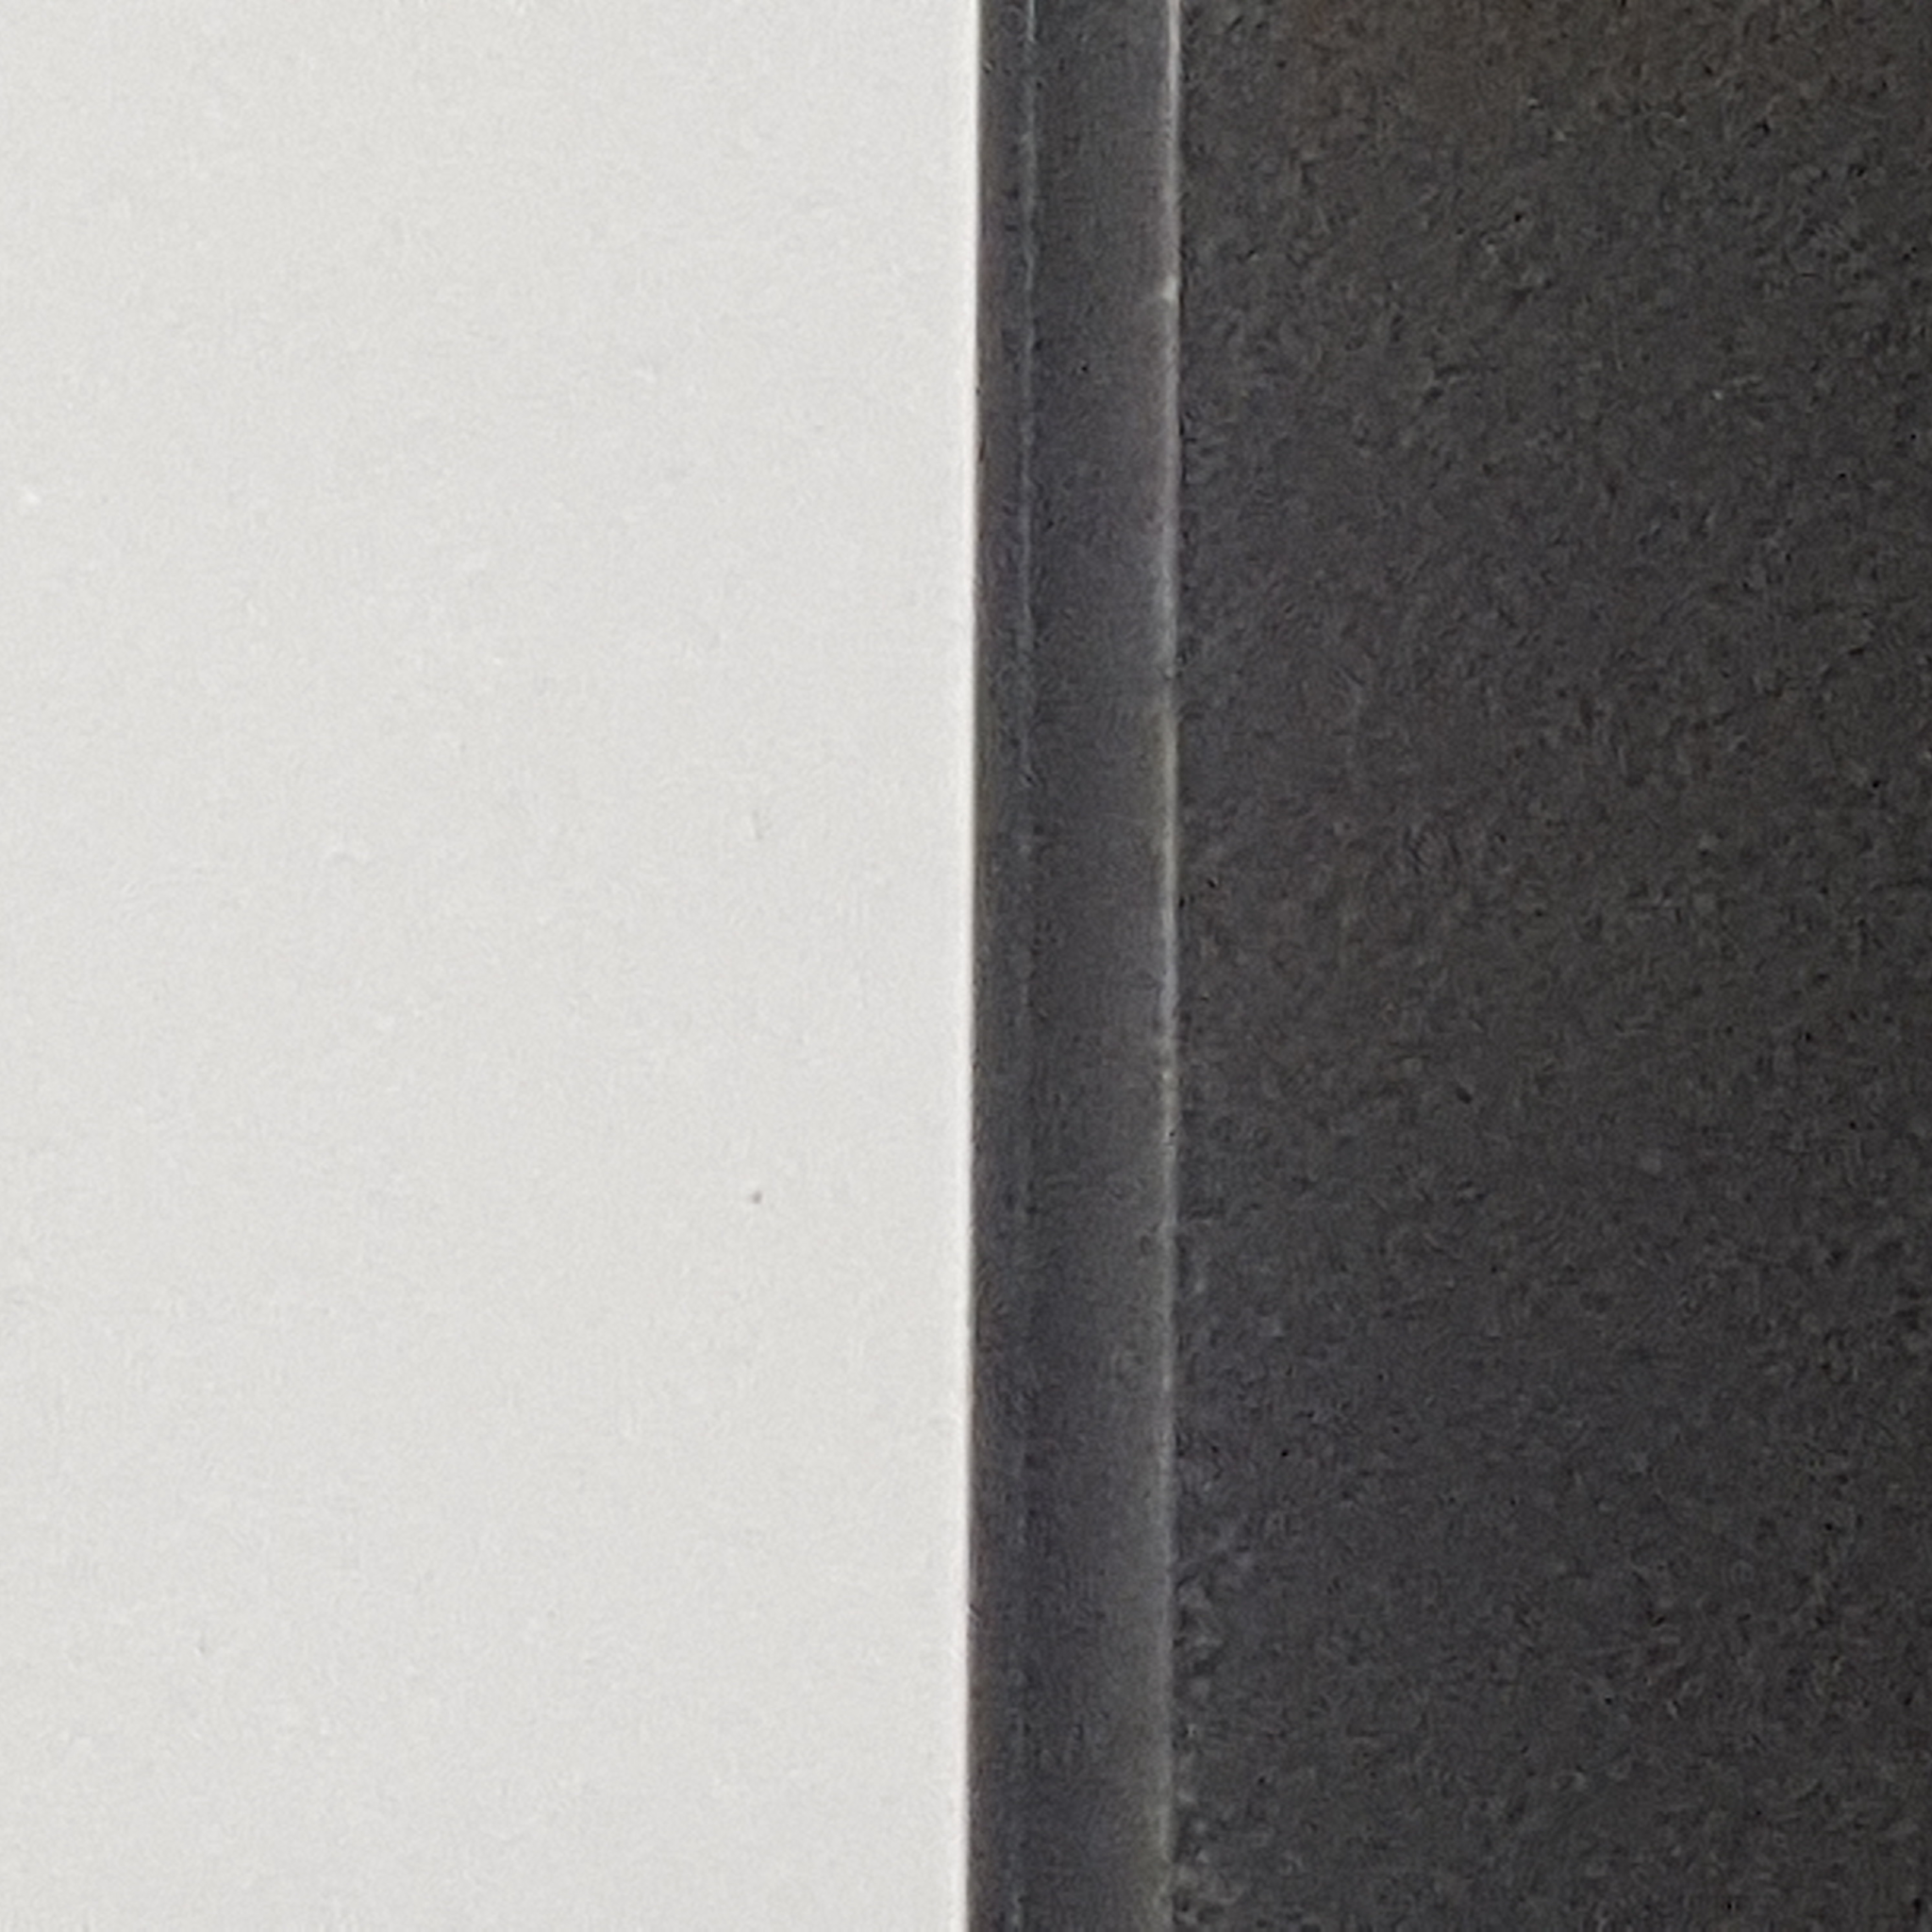
\includegraphics[width=3cm]{images/test2.png} 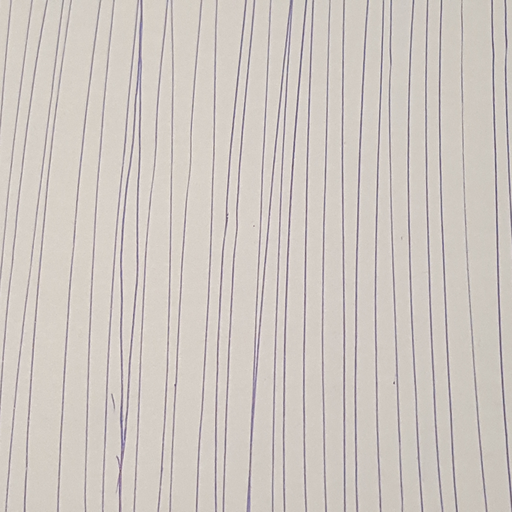
\includegraphics[width=3cm]{images/test1.png} 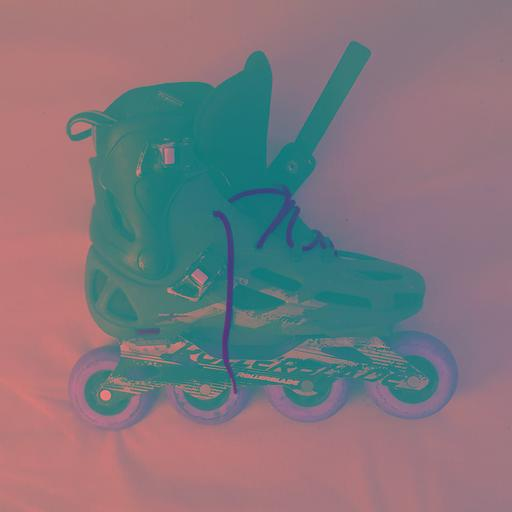
\includegraphics[width=3cm]{images/roller_lab.jpg} \\ 
	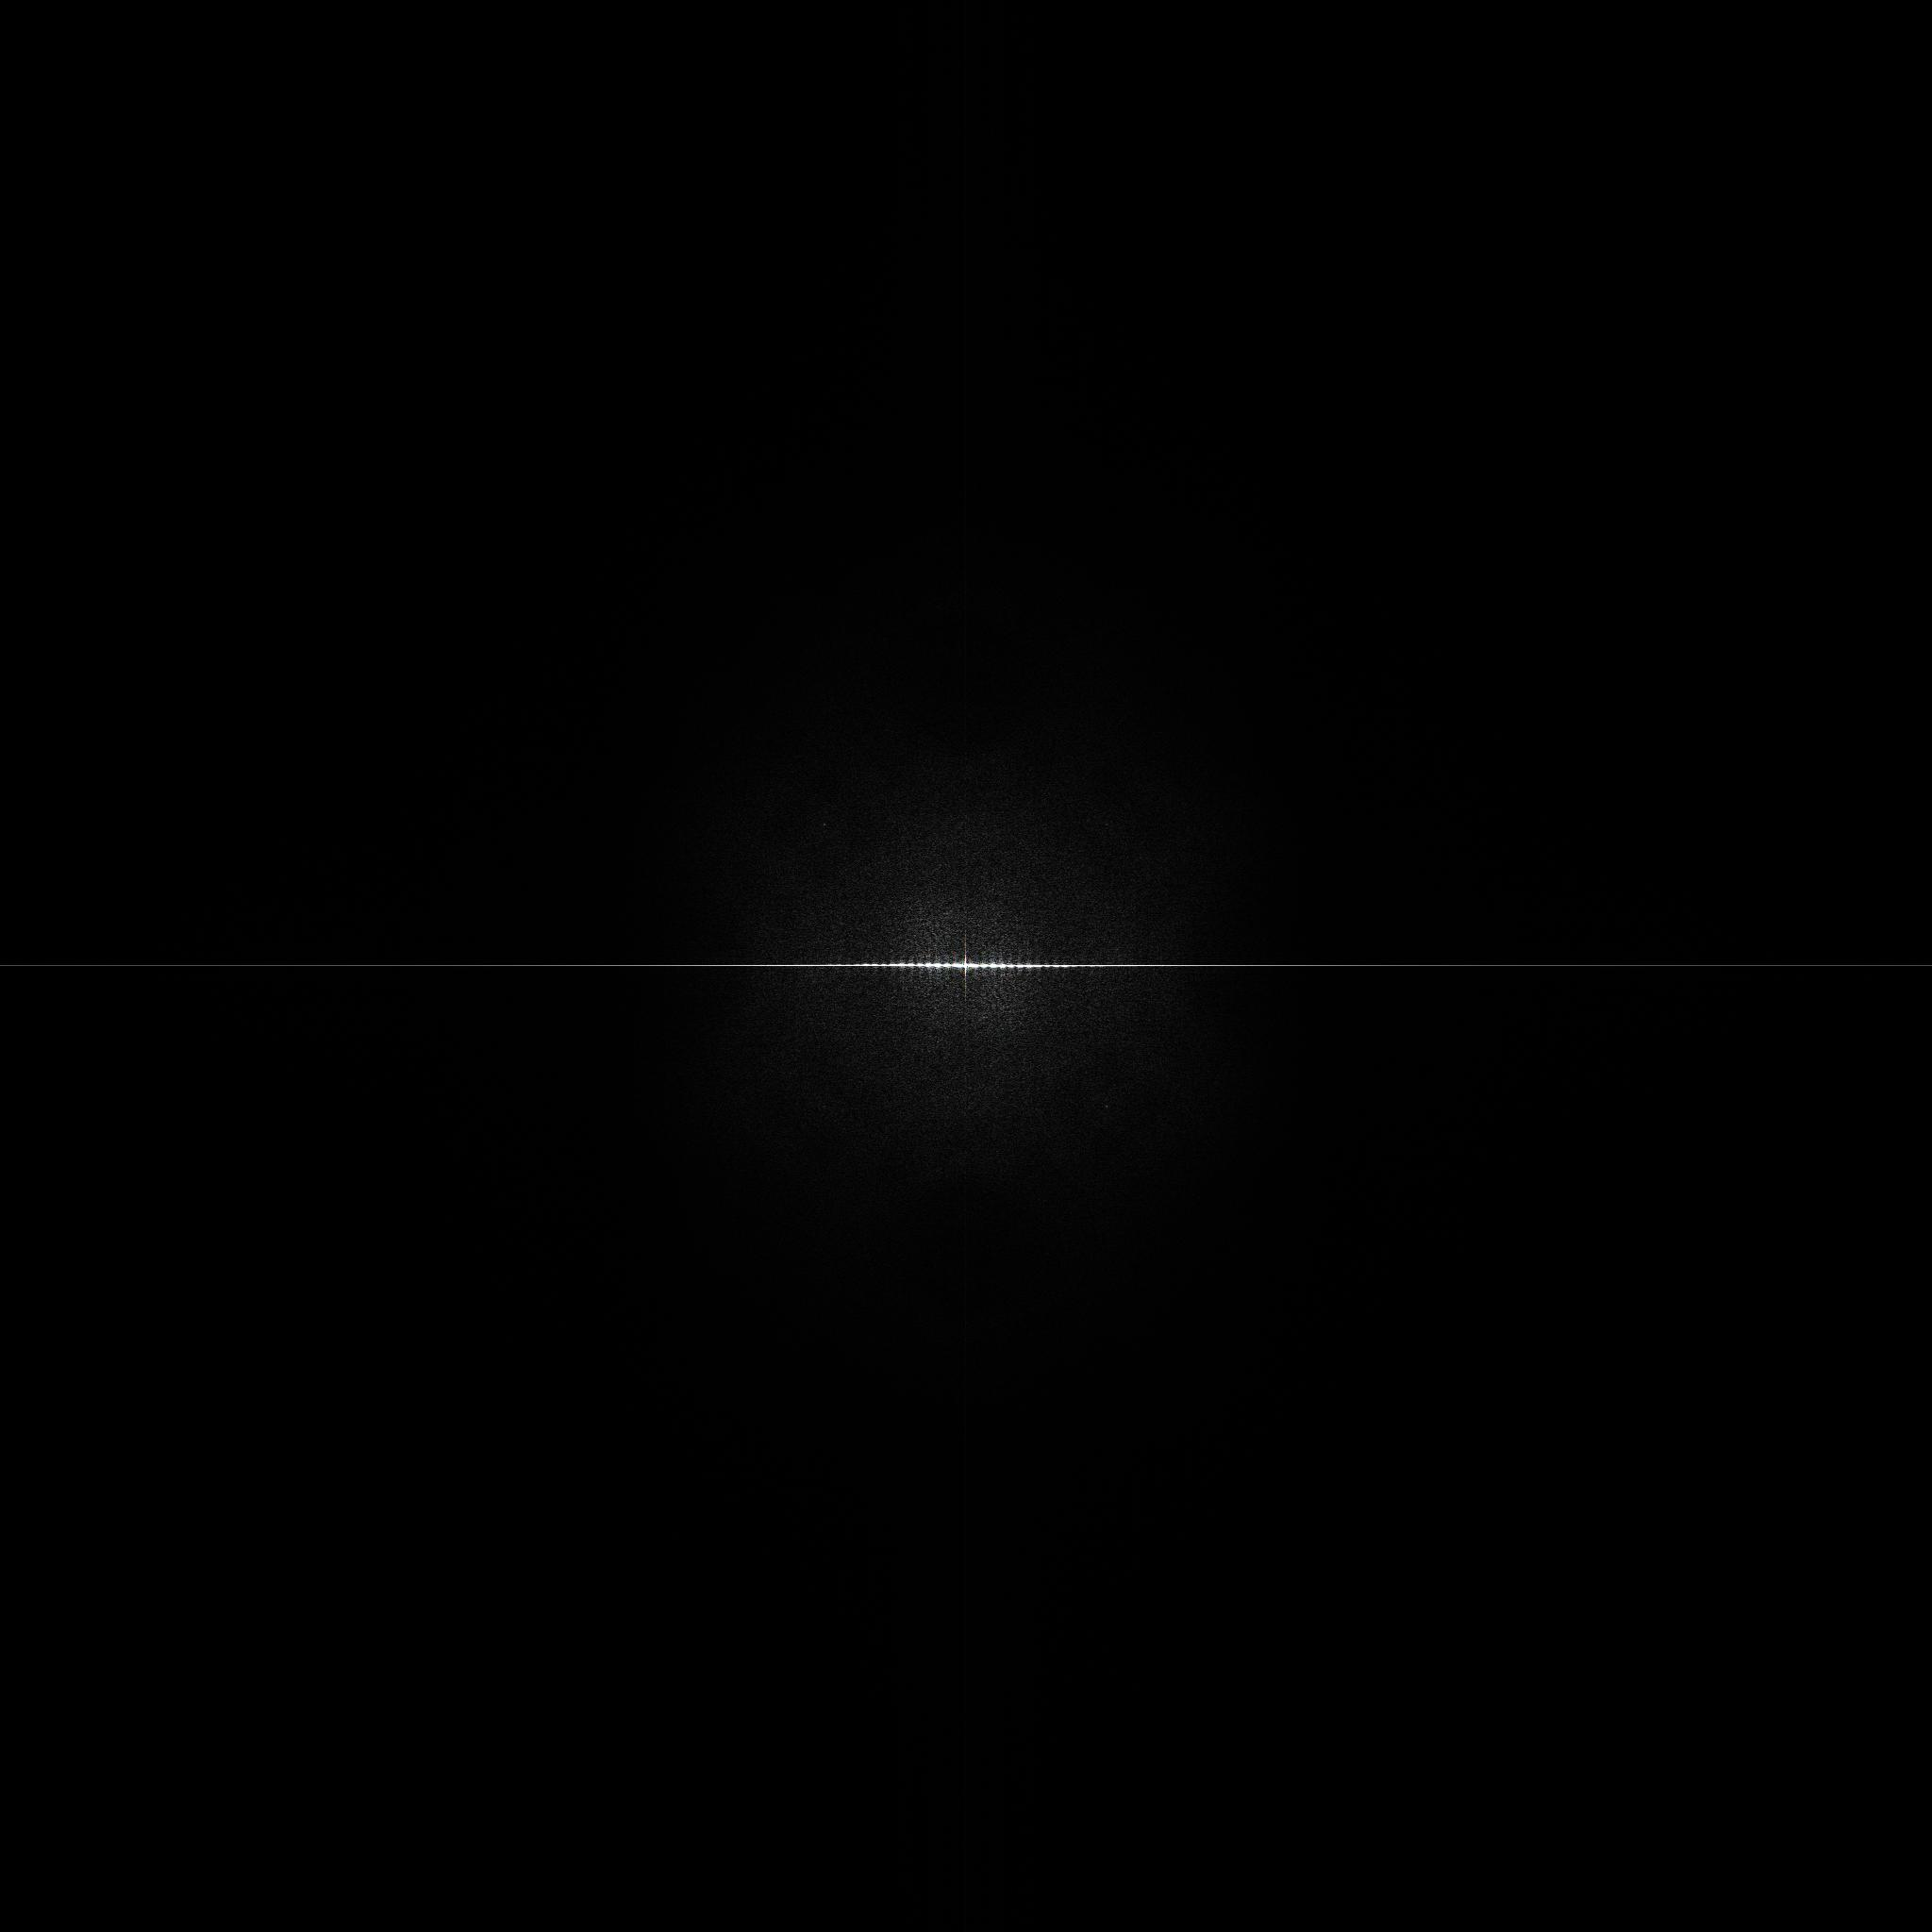
\includegraphics[width=3cm]{images/test2_fft.jpg} 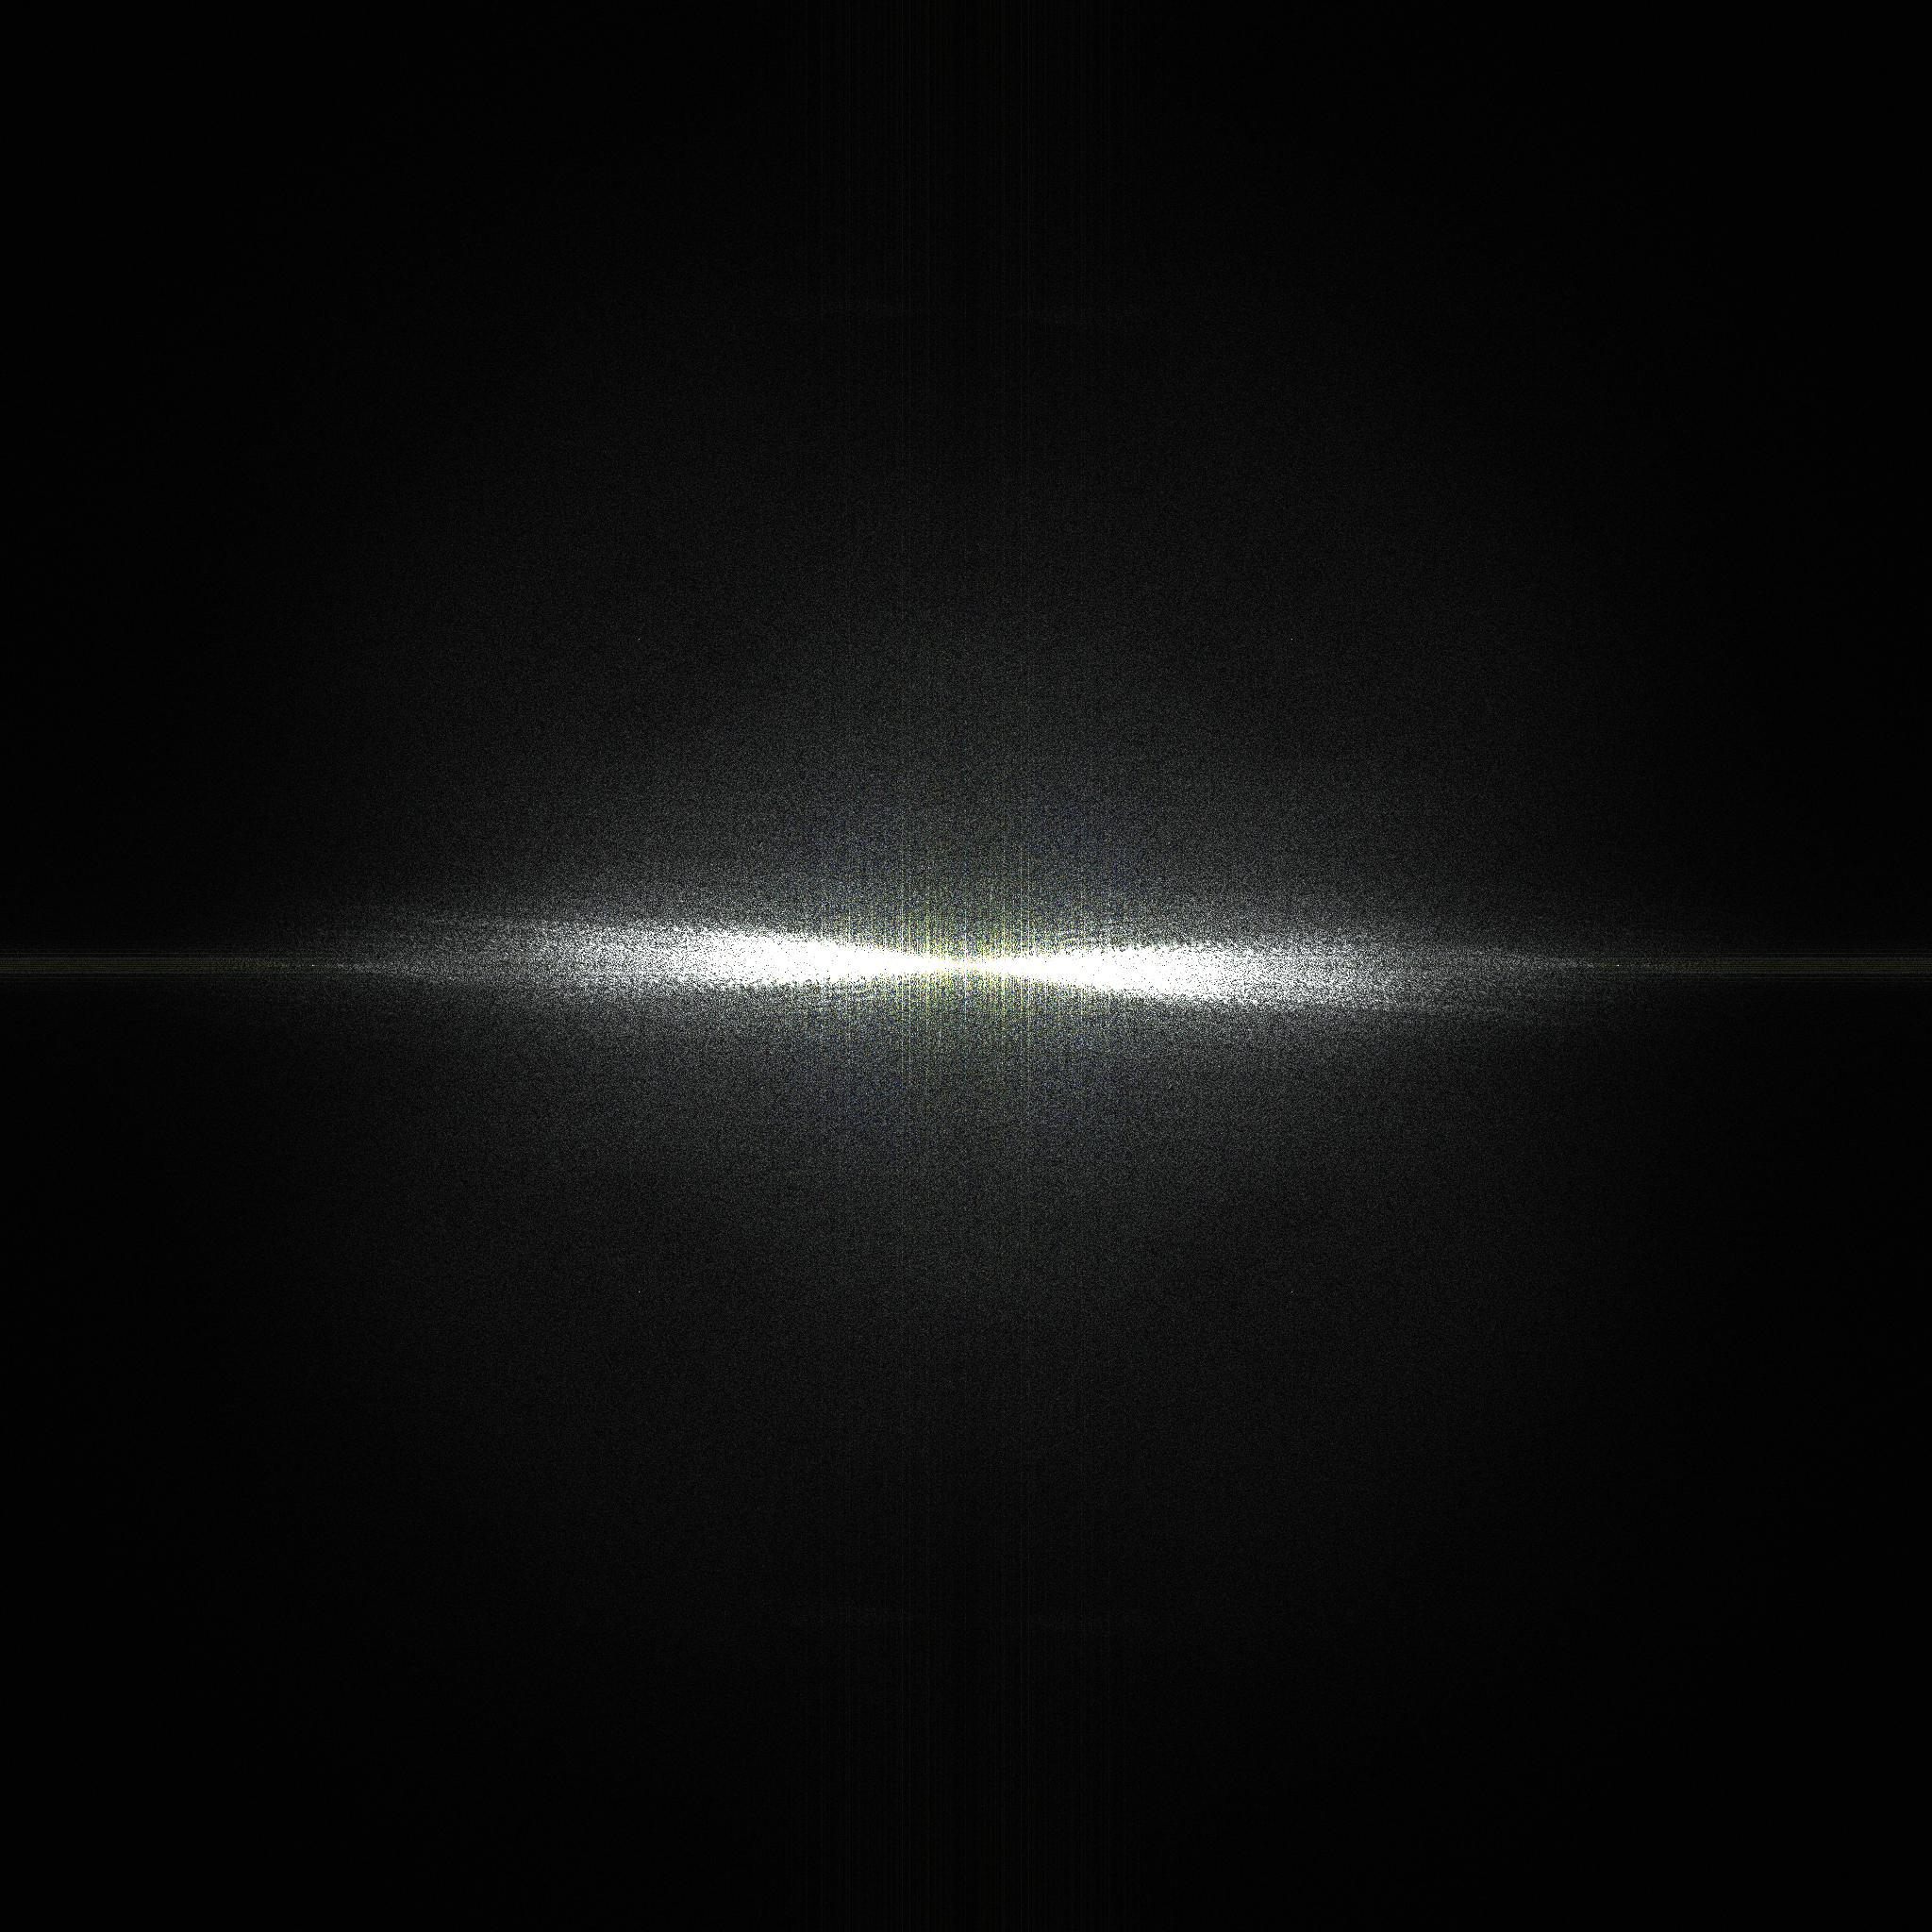
\includegraphics[width=3cm]{images/test1_fft.jpg} 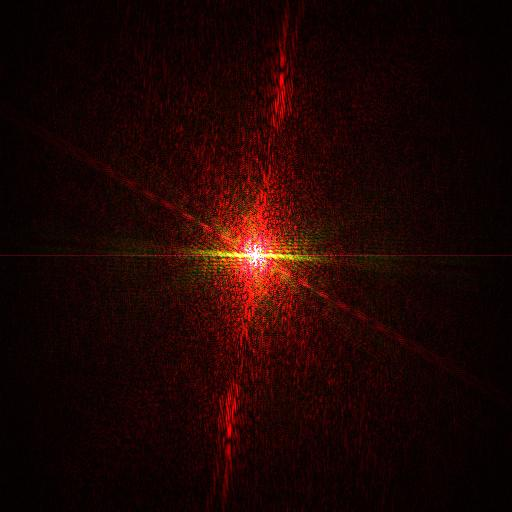
\includegraphics[width=3cm]{images/roller_fft.jpg}	
\end{frame}

\begin{frame}
	\frametitle{\mbox{1\up{er} Filtrage - Domaine fréquentiel - Texture}}
	\framesubtitle{Résultats}
	\begin{figure}
		\centering
		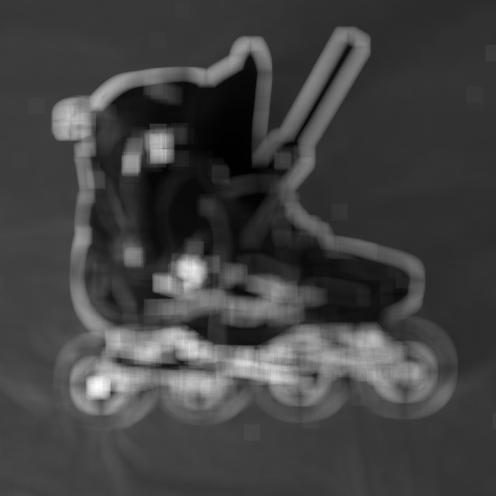
\includegraphics[width=5cm]{images/roller_resp.jpg}
		\caption{taille : 16, $\theta$ : $\frac{\pi}{2}$, $\sigma$ : 4}
	\end{figure}
\end{frame}

\section{Filtrage spatial : Bordures}

\begin{frame}
	\frametitle{\mbox{2\up{ème} Filtrage - Domaine spatial - Bordures}}
	\framesubtitle{Procédé}
	Pour chaque pixel : somme pondérée des pixels du voisinage.\\
	\textbf{Exemple} : gradient simple \\
	\medskip
	\begin{tabular}{|ccc|}
		\hline
		$35$ & $42$ & $27$ \\
		$11$ & $12$ & $14$ \\
		$0$ & $7$ & $4$ \\
		\hline
	\end{tabular}
	\begin{tabular}{|ccc|}
		\hline
		$1$ & $1$ & $1$ \\
		$0$ & $0$ & $0$ \\
		$-1$ & $-1$ & $-1$ \\
		\hline
	\end{tabular}
	\begin{tabular}{|ccc|}
		\hline
		$35$ & $42$ & $27$ \\
		$0$ & $0$ & $0$ \\
		$0$ & $-7$ & $-4$ \\
		\hline
	\end{tabular} \\
	\medskip
	$\longrightarrow$ 93 \\
	\bigskip
	\textbf{Complexité} :
	\begin{itemize}
		\item Spatiale : En place
		\item Temporelle : $\theta(t^2\nu(n^2))$
	\end{itemize}
\end{frame}

\begin{frame}
	\frametitle{\mbox{2\up{ème} Filtrage - Domaine spatial - Bordures}}
	\framesubtitle{Filtre de Canny}
	\begin{columns}
		\begin{column}{5cm}
			Filtre optimal pour les arêtes en "pas"\\
			\textbf{Dérivée d'une gaussienne} :
			$$h(x) = x \cdot e^{-\frac{x^2}{\sigma^2}}$$
		\end{column}
		\begin{column}{5cm}
			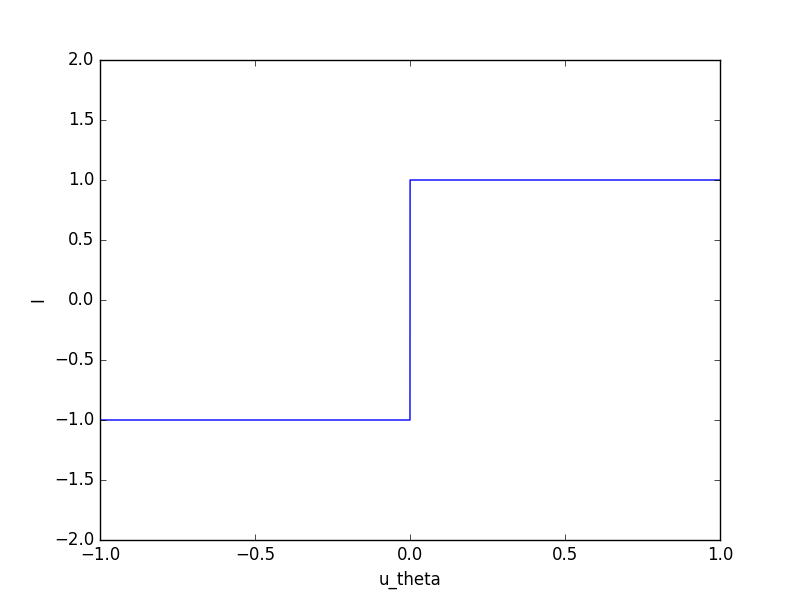
\includegraphics[width=3cm]{images/step.png}\\
			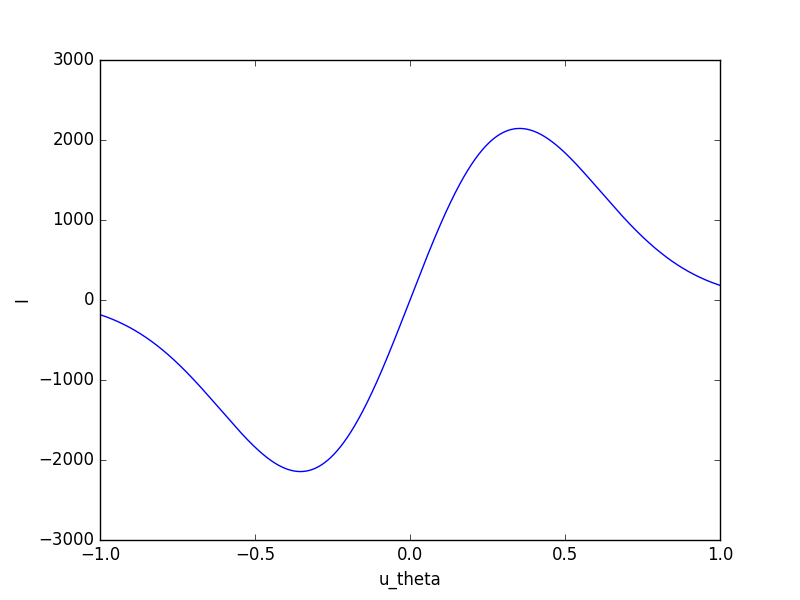
\includegraphics[width=3cm]{images/gaussd1d.png}\\
			
\includegraphics[width=3cm]{images/gaussd.png}
		\end{column}
	\end{columns}
\end{frame}

\begin{frame}
	\frametitle{\mbox{2\up{ème} Filtrage - Domaine spatial - Bordures}}
	\framesubtitle{Résultats}
	\begin{figure}[!h]
		\centering
		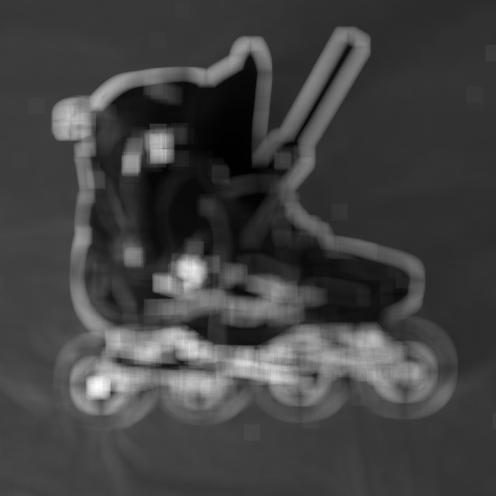
\includegraphics[width=4cm]{images/roller_resp.jpg} \; 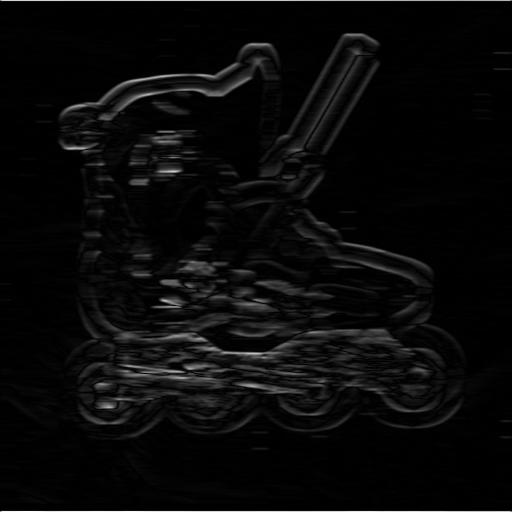
\includegraphics[width = 4cm]{images/roller_filtered.jpg}
		\caption{$\theta$ : $\frac{pi}{2}$, $\sigma$ : 1}
	\end{figure}
\end{frame}

\section{Lissage parabolique}

\begin{frame}
	\frametitle{Lissage parabolique}
	\framesubtitle{Procédé}
	Approximation parabolique du voisinage: $$ax^2 + bx + c = 0$$
	Fonction lissée : $$\frac{c}{\text{distance au max local}} = \frac{c^+}{\left(\frac{|b|}{2a^+}\right)}$$
	Procédé : \\
	\smallskip
	\begin{tabular}{|c|l|r|}
		\hline
		& Opération & complexité \\ \hline
		1 & Génération du voisinage & selon hardware \\ \hline
		2 & Projection des coordonées & $\theta(\nu(t^2))$ \\ \hline
		3 & Etablissement du system & $\theta(t^2 \nu(n^2))$ \\ \hline
		4 & Pivot de gauss & $\theta(t^2 \nu(n^2))$ \\ \hline
		5 & Calcul de la fonction lissée & $\theta(\nu(n^2))$ \\ \hline
		& Total & $\theta(\nu(n^2))$ \\
		\hline
	\end{tabular}
\end{frame}

\begin{frame}
	\frametitle{Lissage parabolique}
	\framesubtitle{Résultats}
	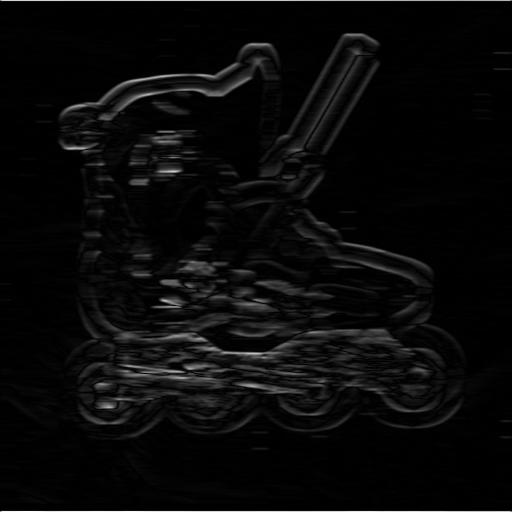
\includegraphics[width=4cm]{images/roller_filtered.jpg} \; 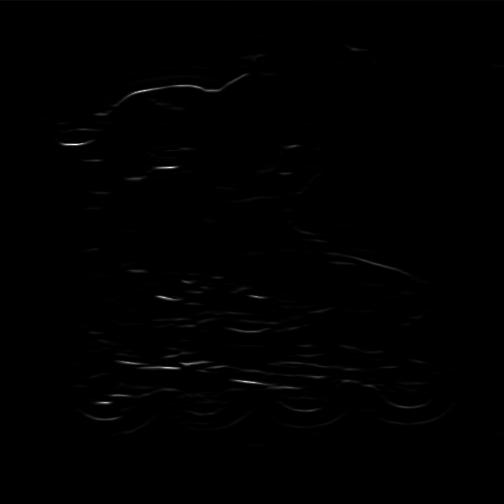
\includegraphics[width=4cm]{images/roller_localised.jpg}
\end{frame}

\section{Sommation des réponses}

\begin{frame}
	\frametitle{Sommation des réponses}
	\framesubtitle{Procédé}
	30 composantes:
	\begin{itemize}
		\item 3 couleurs + 3 couleurs * 4 directions = 15 composantes avant filtrage
		\item pour chaque composante, filtrage par deux filtres de Canny d'écart type 1 et 2 = 30 composantes
	\end{itemize}
	Choix des coefficients de sommation ?\\
	Approche optimale : apprentissage supervisé\\
	Ici : choix empirique
\end{frame}

\begin{frame}
	\frametitle{Sommation des réponses}
	\frametitle{Résultats}
	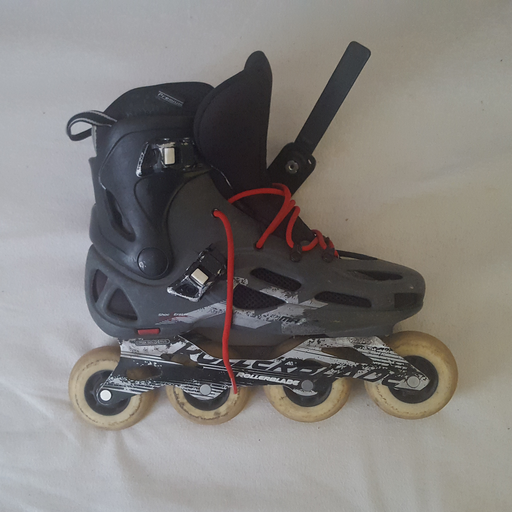
\includegraphics[width=4cm]{images/roller.png} \; 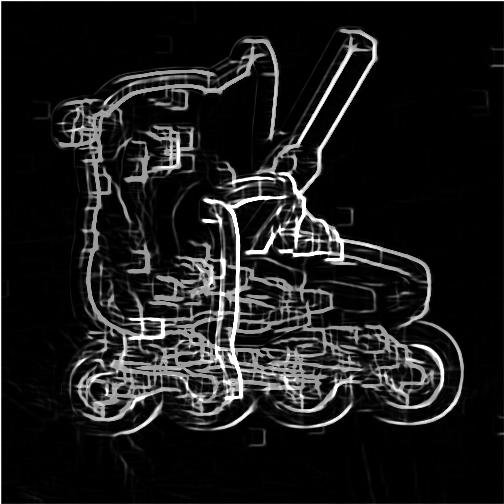
\includegraphics[width = 4cm]{images/roller_res.jpg}
\end{frame}

\section{Seuillage}

\begin{frame}
	\frametitle{Seuillage}
	Conversion en image binaire par seuillage :
	\begin{align}
		\begin{cases}
			1 & \text{si } I>0 \\
			0 & \text{sinon}
		\end{cases}
	\end{align}
	\bigskip
	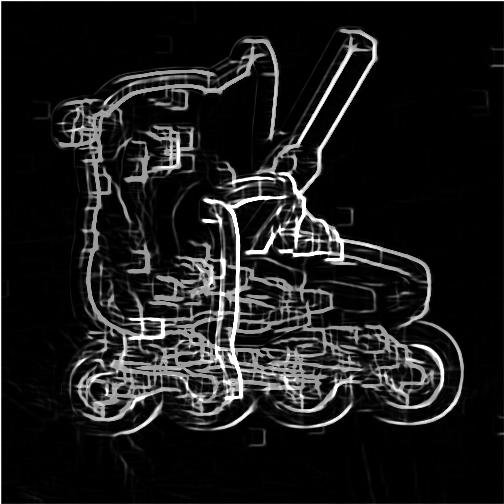
\includegraphics[width=3cm]{images/roller_res.jpg} \; 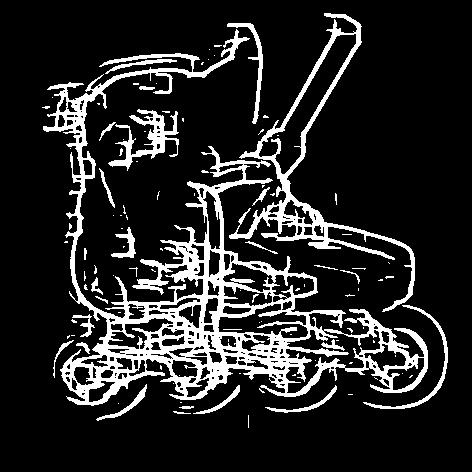
\includegraphics[width=3cm]{images/roller_bin.jpg}
\end{frame}

\section{Opérations topologiques}

\begin{frame}
	\frametitle{Opérations binaires - Topologie}
	\framesubtitle{Définitions}
	Même procédé de filtrage mais sur des images binaires
	\begin{columns}[T]
		\begin{column}{3cm}
			Erosion \\
			\bigskip
			\begin{tabular}{|l|c|r|}
				\hline
				0 & 1 & 0 \\ \hline
				1 & 1 & 1 \\ \hline
				0 & 1 & 0 \\
				\hline
			\end{tabular}
			\begin{tabular}{|l|c|c|c|r|}
				\hline
				0 & 0 & 0 & 0 & 0 \\ \hline
				0 & 1 & 0 & 1 & 0 \\ \hline
				0 & 1 & 1 & 1 & 0 \\ \hline
				1 & 1 & 1 & 1 & 1 \\ \hline
				1 & 1 & 1 & 1 & 1 \\
				\hline
			\end{tabular}
			\begin{tabular}{|l|c|c|c|r|}
				\hline
				0 & 0 & 0 & 0 & 0 \\ \hline
				0 & 0 & 1 & 1 & 0 \\ \hline
				0 & 1 & 1 & 1 & 0 \\ \hline
				0 & 0 & 1 & 1 & 1 \\ \hline
				0 & 0 & 1 & 1 & 1 \\
				\hline
			\end{tabular}
		\end{column}
		\begin{column}{3cm}
			Dilatation \\
			\bigskip
			\begin{tabular}{|l|c|r|}
				\hline
				0 & 0 & 0 \\ \hline
				1 & 1 & 1 \\ \hline
				0 & 0 & 0 \\
				\hline
			\end{tabular}
			\begin{tabular}{|l|c|c|c|r|}
				\hline
				0 & 0 & 0 & 0 & 0 \\ \hline
				0 & 1 & 1 & 1 & 0 \\ \hline
				0 & 0 & 0 & 0 & 1 \\ \hline
				1 & 1 & 1 & 1 & 1 \\ \hline
				1 & 1 & 1 & 1 & 1 \\
				\hline
			\end{tabular}
			\begin{tabular}{|l|c|c|c|r|}
				\hline
				0 & 0 & 0 & 0 & 0 \\ \hline
				0 & 0 & 0 & 0 & 0 \\ \hline
				1 & 1 & 0 & 0 & 0 \\ \hline
				0 & 0 & 0 & 0 & 0 \\ \hline
				0 & 0 & 0 & 0 & 0 \\
				\hline
			\end{tabular}
		\end{column}
		\begin{column}{3cm}
			Fermeture \\
			\bigskip
			Dilatation + Erosion
		\end{column}
	\end{columns}
\end{frame}

\begin{frame}
	\frametitle{Opérations binaires - Topologie}
	\framesubtitle{Résultats}
	\begin{columns}
		\begin{column}{5cm}
			Erosion par : \\
			\medskip
			\begin{tabular}{|l|c|r|}
				\hline
				0 & 1 & 0 \\ \hline
				1 & 1 & 1 \\ \hline
				0 & 1 & 0 \\
				\hline
			\end{tabular} \\
			\medskip
			Fermeture par : \\
			\medskip
			\begin{tabular}{|l|c|c|c|r|}
				\hline
				0 & 0 & 0 & 0 & 0 \\ \hline
				0 & 0 & 0 & 0 & 0 \\ \hline
				1 & 1 & 1 & 1 & 1 \\ \hline
				0 & 0 & 0 & 0 & 0 \\ \hline
				0 & 0 & 0 & 0 & 0 \\
				\hline
			\end{tabular} \\
			\medskip
			Auquel on applique des rotations dans 8 directions différentes
		\end{column}
		\begin{column}{5cm}
			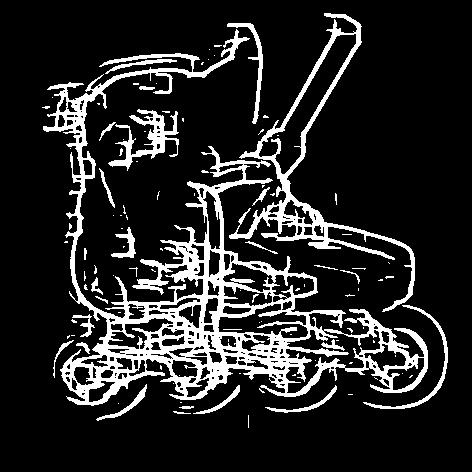
\includegraphics[width=2cm]{images/roller_bin.jpg}\\
			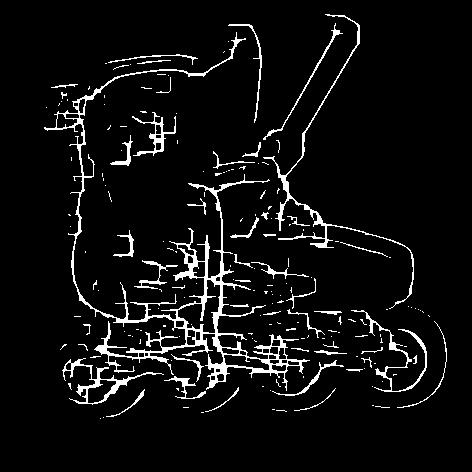
\includegraphics[width=2cm]{images/roller_bin-.jpg}\\
			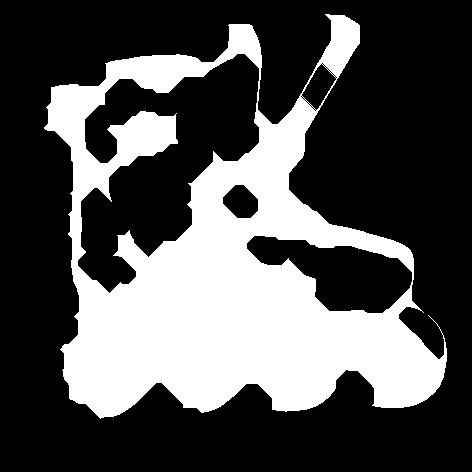
\includegraphics[width=2cm]{images/roller_closedbin.jpg}
		\end{column}
	\end{columns}
\end{frame}

\section{Approximation polygonale}

\begin{frame}
	\frametitle{Approximation polygonale}
	\framesubtitle{Parcours du contour}
	Parcours dans le sens trigonométrique\\
	Départ du pixel le plus en haut\\
	Direction initiale : Bas \\
	Priorités de déplacement : Gauche - Bas - Droite - Haut\\
	\bigskip
	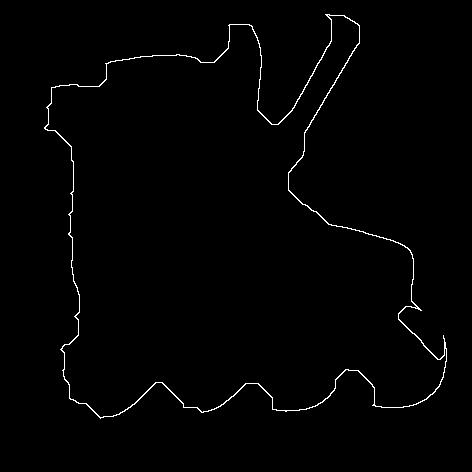
\includegraphics[width=5cm]{images/roller_contour.jpg}
\end{frame}

\begin{frame}
	\frametitle{Approximation polygonale}
	\framesubtitle{Approximation polygonale}
	Initialisation : Point le plus haut - Point le plus bas\\
	Sur chaque segment, successivement :
	\begin{itemize}
		\item Calcul de $D$ distance max du contour au segment
		\item Si $D > \text{seuil}$, on ajoute le point le plus éloigné
		\item Lorsque pour tout segment $D < \text{seuil}$, on sort de la boucle
	\end{itemize}
\end{frame}

\begin{frame}
	\frametitle{Conclusion}
	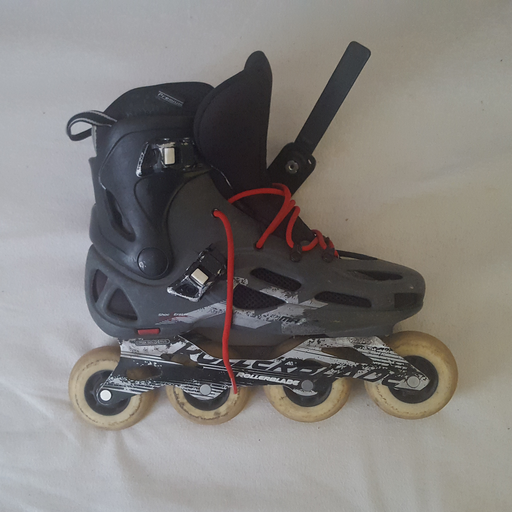
\includegraphics[height=3cm]{images/roller.png} \; 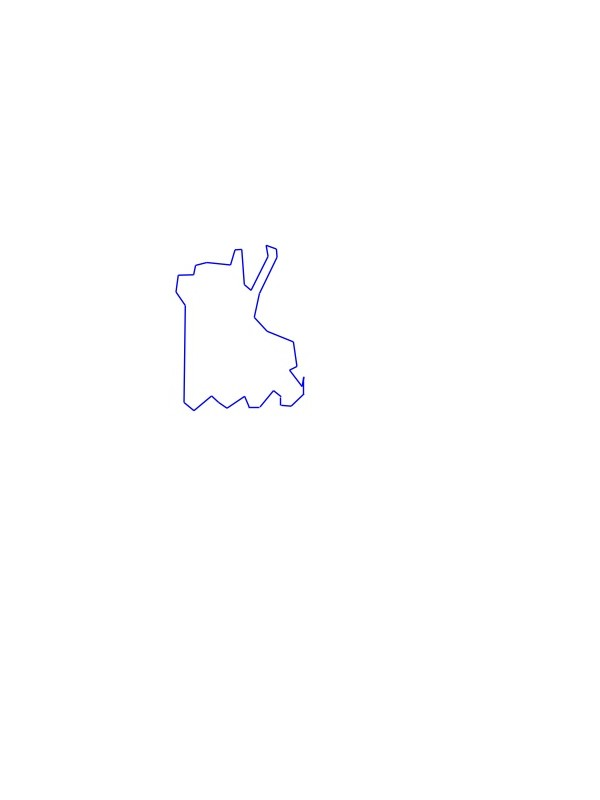
\includegraphics[height=3cm]{images/roller_poly.jpg} \\
	\bigskip
	Précision : moyenne \\
	Temps : moyen $\approx$ 45s\\
\end{frame}

\begin{frame}[allowframebreaks]
	\frametitle{Annexe - Transformée de Fourier rapide}
	Notation :
	\begin{itemize}
		\item $N = 2p$
		\item $n = n_1 + pn_2 \;\;\;\;\; n_1 \in (0, p-1) \;\;\; n_2 \in {0, 1}$
		\item $k = 2k_1 + k_2 \;\;\;\;\; k_1 \in (0, p-1) \;\;\; k_2 \in {0, 1}$
		\item $a = e^{-\frac{2i\pi}{N}}$
	\end{itemize}
	Alors :
	\begin{eqnarray}
		F(u)(k) & = & \sum\limits_{n = 0}^{N-1} u(n) \cdot a^{kn} \\
		F(u)(2k_1 + k_2) & = & \sum\limits_{n_1 = 0}^{1} \sum\limits_{n_2 = 0}^{p-1} u(n_1 + pn_2) \cdot a^{k \cdot (n_1 + pn_2)} \\
		& = & \sum\limits_{n_1 = 0}^{1} \sum\limits_{n_2 = 0}^{p-1} u(n_1 + pn_2) \cdot a^{kn_1} \cdot a^{kpn_2}
	\end{eqnarray}
	De plus :
	$a^{kpn_2} = a^{2p \cdot k_1n_2} \cdot a^{k_2n_1p} = a^{k_2n_1p}$ \\
	Ainsi :
	$F(u)(2k_1 + k_2) = \sum\limits_{n_1 = 0}^{1} a^{kn_1} \cdot \sum\limits_{n_2 = 0}^{p-1} u(n_1 + pn_2) \cdot a^{k_2n_1p}$ \\
	Posons :
	$ v(n_1, k_2) = \sum\limits_{n_2 = 0}^{p-1} u(n_1 + pn_2) \cdot a^{k_2n_1p}$ \\
	Finalement: 
	$F(u)(2k_1 + k_2) = v(0, k_2) + a^{k} \cdot v(1, k_2)$\\
	Le calcul de $v$ est celui d'une transformée de Fourier discrète. On applique récursivement la décomposition
	\bigskip
\end{frame}

\end{document}
